\usetikzlibrary{decorations.pathmorphing}

\section*{Le groupe \texorpdfstring{$GL_n(\R)$}{GLn(R)} et certains de ses sous-groupes}

\[ GL_n(\R) = \{ M \in \mathscr M_n(\R) \mid \det M \neq 0 \}, \quad \text{groupe pour } \times \]
\[ SL_n(\R) = \{ M \in GL_n(\R) \mid \det M = 1 \} \]
\begin{align*}
    GL_n(\Z) &= \{ M \in \mathscr M_n(\Z) \cap GL_n(\R) \mid M^{-1} \in \mathscr M_n(\Z) \} \\
    &= \{ M \in \mathscr M_n(\Z) \mid \det M = \pm 1 \}
\end{align*}

Si $A$ est un anneau commutatif, 
\[
    GL_n(A) = \{ M \in \mathscr M_n(A) \mid \exists N \in \mathscr M_n(A), NM=MI=I \} = \{ M \in \mathscr M_n(A) \mid \det M \in A^\times \}
\]

\begin{proof}
    Si $M \in GL_n(A)$, $MN=I \implies \det M \det N = 1$ donc $\det M \in A^\times$. \\
    Si $\det M \in A^\times$, $M^{-1} = \frac{1}{\det M} {}^t(\text{Com}(M))$.
\end{proof}

\[ SL_n(\Z) = \{ M \in GL_n(\Z) \mid \det M = 1 \} \]

\subsection*{\texorpdfstring{$n=2$}{n=2} : étude de \texorpdfstring{$SL_2(\R)$}{SL2(R)}}

\subsubsection*{Décomposition de Bruhat de \texorpdfstring{$SL_2(\R)$}{SL2(R)}}

\[ B = \left\{ \begin{pmatrix} \alpha & t \\ 0 & 1/\alpha \end{pmatrix} \;\middle|\; \alpha \in \R^*, t \in \R \right\} \text{ est un sous-groupe de } SL_2(\R). \]

\[ \omega = \begin{pmatrix} 0 & -1 \\ 1 & 0 \end{pmatrix} \in SL_2(\R) \]

\begin{theoreme}{}{}
    On peut fabriquer toute matrice de $SL_2(\R) = B \sqcup B \omega B$ \\
    $\hookrightarrow \forall M \in SL_2(\R)$, soit $M \in B$, soit $\exists T_1, T_2 \in B, M = T_1 \omega T_2$.
\end{theoreme}

\begin{proof}
    Cela repose sur le fait que $B$ agit sur $\R^2 \setminus \{(0,0)\}$.
    \[ 
        \fonction{ }{B \times (\R^2 \setminus \{(0,0)\})}{\R^2 \setminus \{(0,0)\}}{(M, X)}{MX} 
    \]

    \uline{Orbites} : soit $e_1 = \begin{pmatrix} 1 \\ 0 \end{pmatrix}$
    \[ 
        B e_1 = \left\{ \begin{pmatrix} \alpha & t \\ 0 & 1/\alpha \end{pmatrix} \begin{pmatrix} 1 \\ 0 \end{pmatrix} = \begin{pmatrix} \alpha \\ 0 \end{pmatrix} \right\} 
    \]

    \begin{center}
    \begin{tikzpicture}[scale=1.5]
        % Axes
        \draw[->] (-2.5,0) -- (2.5,0);
        \draw[->] (0,-1) -- (0,1);
        
        % Label e1
        \draw (1, 0.1) -- (1, -0.1) node[below] {$e_1$};
        
        % Sur lignage de l'orbite (axe x privé de 0)
        \draw[line width=1.5pt, purple] (-2.5,0) -- (-0.05,0);
        \draw[line width=1.5pt, purple] (0.05,0) -- (2.5,0);
        \node[purple, above] at (1.5, 0.1) {$B e_1$};
        
        % Origine exclue visuellement
        \node at (0,0) [circle, fill=white, inner sep=1pt, draw=black] {}; 
    \end{tikzpicture}
    \end{center}
\end{proof}

Soit $e_2 = \begin{pmatrix} 0 \\ 1 \end{pmatrix}$. 
\[ B e_2 = \left\{ \begin{pmatrix} t \\ 1/\alpha \end{pmatrix} \mid \alpha \neq 0, t \in \R \right\} \]

\begin{center}
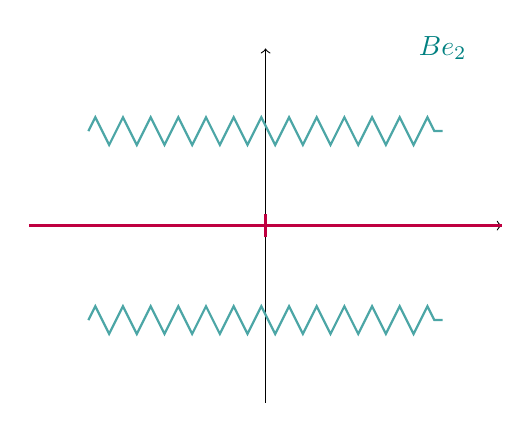
\begin{tikzpicture}[scale=1.5]
    % Axes
    \draw[->] (-2,0) -- (2,0);
    \draw[->] (0,-1.5) -- (0,1.5);
    
    % Label Be2
    \node[teal, font=\bfseries] at (1.5, 1.5) {$B e_2$};
    
    % Gribouillages verts symbolisant le plan privé de l'axe x
    \draw[teal!70, thick, decorate, decoration={zigzag, segment length=10pt, amplitude=5pt}] (-1.5, 0.8) -- (1.5, 0.8);
    \draw[teal!70, thick, decorate, decoration={zigzag, segment length=10pt, amplitude=5pt}] (-1.5, -0.8) -- (1.5, -0.8);
    
    % Croix/Séparation violette
    \draw[purple, very thick] (-2,0) -- (2,0);
    \draw[purple, very thick] (0,-0.1) -- (0,0.1); 
\end{tikzpicture}
\end{center}

\[ \text{Stab}(e_1) = B_{e_1} = \{ M \in B \mid M e_1 = e_1 \} = \left\{ \begin{pmatrix} 1 & * \\ 0 & 1 \end{pmatrix} \right\} = U. \]

Soit $M \in SL_2(\R)$.
\begin{itemize}
    \item Si $M e_1 \in B e_1$, $\exists b \in B, M e_1 = b e_1$ et $b^{-1} M e_1 = e_1$. \\
    Donc $b^{-1} M \in B_{e_1} \subset B$, donc $M \in B$.

    \item $2^{\text{ème}}$ cas : Si $M e_1 \in B e_2$. Or $\omega = \begin{pmatrix} 0 & -1 \\ 1 & 0 \end{pmatrix}$, $e_2 = \omega e_1$. \\
    Donc $M e_1 \in B \omega e_1$. \\
    $\exists b, M e_1 = b \omega e_1$ et donc $\omega^{-1} b^{-1} M e_1 = e_1$. \\
    Donc $b' = \omega^{-1} b^{-1} M \in B_{e_1} \subset B$. \\
    Donc $M = b \omega b' \in B \omega B$.
\end{itemize}

Par l'absurde : si $M \in B \cap B \omega B$, alors $M = b = b_1 \omega b_2$ \\
et donc $\omega = b_1^{-1} b b_2^{-1} \in B \implies$ absurde (car un élément de $B$ a un 0 en bas à gauche, pas $\omega$).
\qed

\begin{corollaire}{}{}
    $B$ est un sous-groupe maximal de $SL_2(\R)$. \\
    Soit $G$ un sous-groupe tq $B \subset G \subset SL_2(\R)$ alors $G=B$ ou $G=SL_2(\R)$.
\end{corollaire}

\begin{proof}
    Supposons $\exists M \in G \setminus B$. \\
    Donc $\exists b_1, b_2 \in B$ tq $M = b_1 \omega b_2$ et donc $\omega = \underbrace{b_1^{-1}}_{\in G} \underbrace{M}_{\in G} \underbrace{b_2^{-1}}_{\in G} \in G$. \\
    Et $\forall b, b'$, $b \omega b' \in G$ donc $B \omega B \subset G$ et $B \subset G$. \\
    $SL_2(\R) \subset G$.
\end{proof}

\section*{Décomposition KAN}

\[ K = \left\{ \begin{pmatrix} \cos \theta & -\sin \theta \\ \sin \theta & \cos \theta \end{pmatrix}, \theta \in \R \right\} \quad A = \left\{ \begin{pmatrix} x & 0 \\ 0 & 1/x \end{pmatrix} \mid x \in \R^* \right\} \]
\[ N = \left\{ \begin{pmatrix} 1 & \lambda \\ 0 & 1 \end{pmatrix} \mid \lambda \in \R \right\}. \quad \text{Alors } K, A, N \subset SL_2(\R). \]

\section*{Théorème KAN}

\begin{theoreme}{KAN}{}
    \uindent{Version algébrique} (1) $\forall M \in SL_2(\R), \exists! (k, a, n) \in K \times A \times N$ tel que $M = kan$. \\
    
    \uindent{Version topologique} (2) L'application 
    $\fonction{\phi}{K \times A \times N}{SL_2(\R)}{(k, a, n)}{kan}$
    est un homéomorphisme, c'est-à-dire que $\phi^{-1}$ est continue.
\end{theoreme}

\begin{proof}
    Soit $\mathbb{H} = \{ z \in \C \mid \Im z > 0 \}$. \\
    $SL_2(\R)$ agit sur $\mathbb{H}$ de la façon suivante : 
    \[ 
        \fonction{}{SL_2(\R) \times \mathbb{H}}{\mathbb{H}}{\left(\begin{pmatrix} a & b \\ c & d \end{pmatrix}, z\right)}{\frac{az+b}{cz+d}} 
    \]

    Si $a \in A, a = \begin{pmatrix} x & 0 \\ 0 & 1/x \end{pmatrix}$ donc $a \cdot z = \frac{xz}{1/x} = x^2 z$. \\
    $\rightarrow A$ agit par homothéties de rapport $> 0$.

    Si $n \in N, n = \begin{pmatrix} 1 & \lambda \\ 0 & 1 \end{pmatrix}$, $n \cdot z = \frac{1 \cdot z + \lambda}{1} = z + \lambda$. \\
    $\rightarrow N$ agit par translation horizontale.

    \uline{Calcul du stabilisateur de $i$} :
    \[ \text{Stab}(i) = \left\{ \begin{pmatrix} a & b \\ c & d \end{pmatrix} \in SL_2(\R) \;\middle|\; \frac{ai+b}{ci+d} = i \right\} \]
    $\frac{ai+b}{ci+d} = i \iff ai+b = -c+di \iff b = -c \text{ et } a = d$.
    \[ 
        \text{Stab}(i) = \left\{ \begin{pmatrix} a & b \\ -b & a \end{pmatrix} \;\middle|\; a^2 + b^2 = 1 \right\} = SO_2(\R) = K 
    \]

    Soit $M \in SL_2(\R)$. Posons $z = M^{-1} \cdot i \in \mathbb{H}$.

    \begin{center}
    \begin{tikzpicture}[scale=2]
        % Axes
        \draw[->] (-1.5,0) -- (2,0) node[right] {$\R$};
        \draw[->] (0,-0.2) -- (0,2.5) node[above] {$i\R$};
        
        % Point i
        \fill (0,1) circle (1pt) node[left] {$i$};
        \draw (0.1,1) -- (-0.1,1);

        % Point z
        \coordinate (z) at (1.2, 1.8);
        \fill (z) circle (1pt) node[above right] {$z = M^{-1} \cdot i$};
        
        % Point intermédaire nz
        \coordinate (nz) at (0, 1.8);
        \fill (nz) circle (1pt) node[left] {$nz$};

        % Flèche n (translation)
        \draw[->, thick, sectionblue] (z) -- (nz) node[midway, above] {$n$};
        
        % Flèche a (homothétie)
        \draw[->, thick, redbox] (nz) -- (0, 1.1) node[midway, left] {$a$};

        % Annotations
        \node[right, align=left, font=\small] at (1.5, 1) {$\exists n \in N, nz \in i\R$ \\ $\exists a \in A, anz = i$};
    \end{tikzpicture}
    \end{center}

    On a $a n z = i$ donc $a n M^{-1} \cdot i = i$. \\
    Donc $a n M^{-1} \in \text{Stab}(i) = K$. \\
    $\exists k' \in K, a n M^{-1} = k' \implies M = (k')^{-1} a n$. \\
    En posant $k = (k')^{-1}$, on a $M = k a n$.

    \uline{Unicité} : Supposons $k_1 a_1 n_1 = k_2 a_2 n_2$. \\
    Alors $k_2^{-1} k_1 = a_2 n_2 n_1^{-1} a_1^{-1}$. \\
    Appliquons ceci à $i$ :
    \[ k_2^{-1} k_1 \cdot i = i \quad (\text{car } K = \text{Stab}(i)) \]
    Donc $a_2 n_2 n_1^{-1} a_1^{-1} \cdot i = i$.
    
    Or l'action de $N$ affecte la partie réelle et celle de $A$ la partie imaginaire de manière unique pour ramener sur $i$.
    On en déduit que $n_2 n_1^{-1} = I$ et $a_2 a_1^{-1} = I$.
    D'où $n_1 = n_2$, $a_1 = a_2$ et donc $k_1 = k_2$.

    \uline{Continuité de l'inverse} : \\
    $(k, a, n) \mapsto kan$. On veut montrer que l'application réciproque est continue. \\
    Soit $(M_j)$ une suite de matrices telle que $M_j \tend{j}{\infty} M \in SL_2(\R)$. \\
    On écrit $M_j = k_j a_j n_j$ et $M = k a n$. On veut montrer que $k_j \to k$, $a_j \to a$, $n_j \to n$. \\
    (La preuve utilise la continuité des opérations algébriques et l'unicité de la décomposition).

et on veut $k_j \to k$, $a_j \to a$ et $n_j \to n$.

$K$ est un sous groupe compact de $SL_2(\R)$. \\
Donc $k_j \to k \iff k$ seule valeur d'adhérence de $(k_j)$.

Soit $k_{\sigma(j)} \to k'$ une valeur d'adhérence.
\[ k_{\sigma(j)} a_{\sigma(j)} n_{\sigma(j)} \to k a n \]

\[ 
    \underbrace{a_{\sigma(j)} n_{\sigma(j)}}_{\substack{\in AN \\ \text{fermé de } SL_2(\R)}} = 
    \underbrace{k_{\sigma(j)}^{-1}}_{\to (k')^{-1}} 
    \underbrace{k_{\sigma(j)} a_{\sigma(j)} n_{\sigma(j)}}_{\to k a n} 
    \limit{j}{\infty} 
    \underbrace{(k')^{-1} k a n}_{\in AN} 
\]

Et donc par unicité de la décomposition de KAN, $(k')^{-1} k = I$, donc $k = k'$.
\end{proof}